\chapter{Planar Nef Polyhedra}

A planar Nef polyhedron is any set that can be obtained from the open
halfspaces by a finite number of set complement and set intersection
operations. The set of Nef polyhedra is closed under the Boolean set
operations.  The following data structure realizes two-dimensional
Nef polyhedra and offers a large set of binary and unary set
operations. The underlying set operations are realized by an efficient
and complete algorithm for the overlay of two Nef polyhedra. The
algorithm is efficient in the sense that its running time is bounded
by the size of the inputs plus the size of the output times a
logarithmic factor. The algorithm is complete in the sense that it can
handle all inputs and requires no general position assumption.


\begin{figure}[htbp]
\begin{ccTexOnly}
\begin{center}
\scalebox{0.5}{\includegraphics{Nef_2_ref/halfplane.ps}}
\scalebox{0.5}{\includegraphics{Nef_2_ref/complex.ps}}
\end{center}
\end{ccTexOnly}
\caption{Two nef polyhedra in the plane. A halfspace on the left and a
complex polyhedron on the right. Note that the points on the squared
boundary are at infinity.}
\label{extsegs}    
\begin{ccHtmlOnly}
<CENTER>
<IMG BORDER=0 SRC="./halfplane.gif" ALIGN=center
ALT="a halfplane">
<IMG BORDER=0 SRC="./complex.gif" ALIGN=center
ALT="a complex polyhedron">
</CENTER>
\end{ccHtmlOnly}
\end{figure}
